\section{Methods} \label{section:methods}

\subsection{Current Implementation}

The current implementation is a combination of two main areas of research with a motivation to accelerate reinforcement learning. The reinforcement learning algorithm used in this research is the Twin Delayed Deep Deterministic Policy Gradient (TD3) which has shown better performance compared to its widely used predecessor DDPG. The two areas of focus in this research will be, combining behavior cloning with reinforcement learning which is the combination of BC + TD3 and designing an optimal reward function. \\

\subsection{Loss Functions}

\subsection{Q-Filter}

\subsection{Replay Buffer}

\subsection{Demonstrations}

\subsection{Training Strategy}

\subsection{Reward Design}

\subsection{Deep Learning Specifications}

\subsection{Hyperparameters List}

\subsection{Algorithm Pseudocode}

\subsection{Simulation Environments $\&$ Task Description}

\begin{figure}[h!]
    \centering
    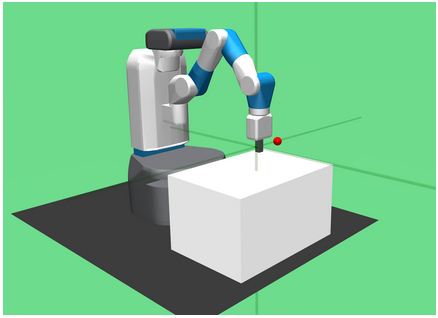
\includegraphics{images/FR.png}
    \caption{Simple Representation of the Fetch Reach Task}
    \label{fig:FR}
\end{figure}

\begin{figure}[h!]
    \centering
    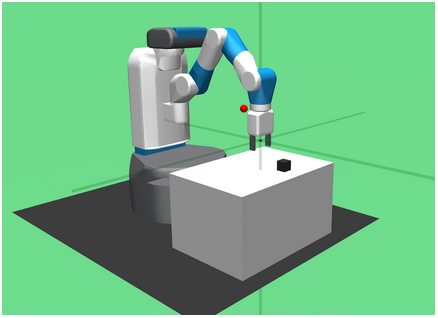
\includegraphics{images/FPAP.png}
    \caption{Simple Representation of the Fetch Pick And Place Task}
    \label{fig:FPAP}
\end{figure}

\begin{figure}[h!]
    \centering
    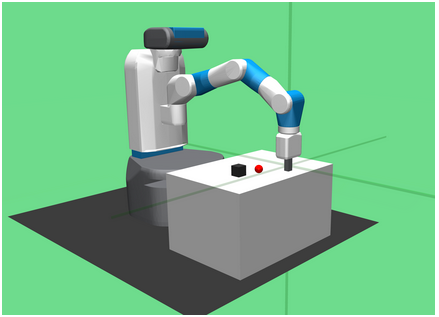
\includegraphics{images/FP.png}
    \caption{Simple Representation of the Fetch Push Task}
    \label{fig:FP}
\end{figure}

\begin{figure}[h!]
    \centering
    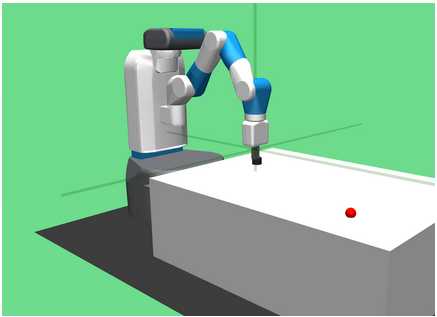
\includegraphics{images/FS.png}
    \caption{Simple Representation of the Fetch Slide Task}
    \label{fig:FS}
\end{figure}

The current implementation



